\section{Introduction}
\label{sec:intro}

Human interaction with computers is one of the most fundamental components in today's complex systems, and interfaces are crucial for the interactions. In a traditional setting, a user accesses a computer (we call them the \emph{host} systems for the rest of this paper), most commonly a PC to configure remote end systems such as a web server. Systems illustrated in Figure~\ref{fig:motivation} such as critical infrastructures, automation systems, financial transaction, and many more day to day services rely on human input and proper understanding of output from the server. Hence, the correctness of the input and output is of uttermost importance. And most of these systems are hosted remotely and provide a web-based UI. The complexity of modern operating systems and software has proven that host systems largely remain vulnerable to attacks. A compromised host threatens the integrity and the confidentiality of any interaction between the user and a remote server. It can easily alter the data transferred from the user to the remote server or trick the user to perform unintended actions, or observe any sensitive communication going through.

%Human interaction with computers is one of the most fundamental components in today's complex systems, and interfaces are crucial for the interactions. All computing devices (we call them the \emph{host} systems), such as desktop computers, smartwatches, embedded devices provide some input and output mechanisms via the user interfaces (UI) where the users can provide input to the computers and retrieve information. These input interfaces are the embodiments of the human-computer interaction (HCI). Critical infrastructures, automation systems, financial transaction, and many more day to day services rely on human input, and the correctness of the input is of uttermost importance. The complexity of modern operating systems and software has proven that computers largely remain vulnerable to attacks. A compromised computer threatens the integrity and the confidentiality of any interaction between the user and a remote server. It can easily alter the data transferred from the user to the remote server or trick the user to perform unintended actions, or observe any sensitive communication going through. Therefore, the necessity of \emph{trusted paths} for IO between the user and remote servers is essential. The trusted path is a concept that in-theory solves the problem of user IO security between the user and the end-system. The trusted path provides a secure channel between the user (HID) to the end system, and this end system could be a remote server or a local computer. 

\begin{figure}[t]
\centering
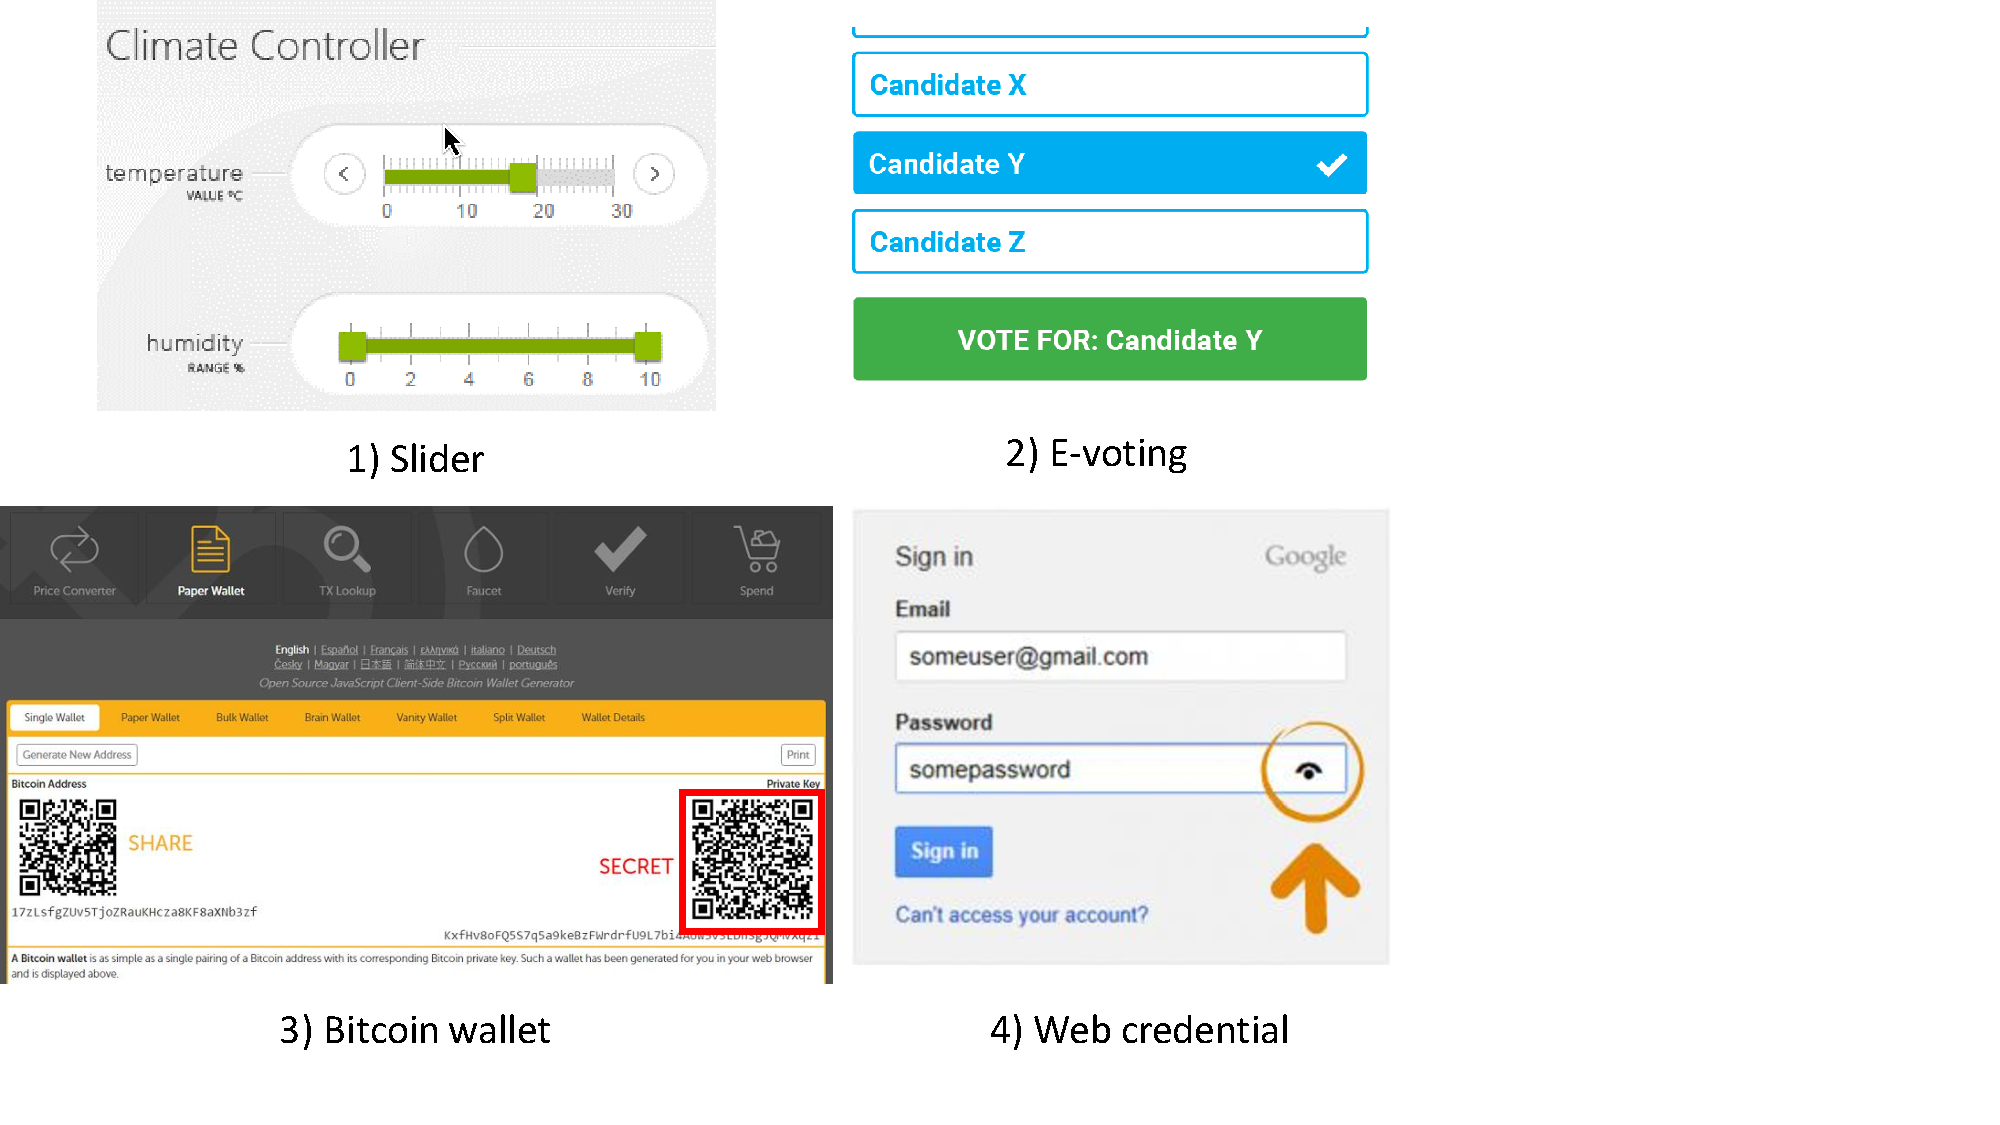
\includegraphics[trim={0 1cm 10cm 0}, clip, width=\linewidth]{motivation.pdf}
\caption{\textbf{Motivating examples.} 1) Pointer based UI elements that sets parameters to remote safety-critical device, 2) E-voting where the voting privacy and integrity is critical, 3) Financial transactions such as bitcoin wallet that shows sensitive information such as the user's private key and 4) web applications that provide an option for the user to reveal credentials.}
\spacesave
\label{fig:motivation}
\centering
\end{figure}


IO operation between the user and a remote server in the presence of an untrusted host is a long-standing problem. \emph{Trusted path} provides a secure channel between the user (HID) and the end-point where end-point is typically a trust worthy application running on the host. Trusted path ensures that input from the user is reached to the intended application and all the outputs are generated by the legitimate application. Trusted path to the local host is a well-researched area where many solutions focus on using trusted software components such as a trusted hypervisor. Sel4~\cite{klein2009sel4} is a functional hypervisor that is formally verified and has a kernel size of only $8.4k$ lines of code. In work done by Zhou et al.~\cite{zhou2012building}, the authors proposed a generic trusted path on $x86$ systems in pure hypervisor-based design. SGXIO~\cite{weiser2017sgxio} employs both hypervisor and trusted execution environment (TEE) such as Intel SGX. %For the remote variant, VButton~\cite{li2018vbutton} uses ARM TrustZone to overlay buttons on the mobile devices that confirm if the user taps on a specific button. 

However, when we consider an untrusted host, trusted path to the local host does not provide any advantage. In such a attacker model, it is crucial to ensure a trusted path from the user to a trusted remote server. Remote trusted path variant is non-trivial as typically all the IO operations are mediated by the operating system, device drivers, etc. Usage of an external trusted device is also another way to contract a trusted path. Transaction confirmation devices~\cite{filyanov2011uni,weigold2011secure} leverages on external device to confirm the input parameters. This allows the user to review her input data on a separate trusted device that is physically separated from the untrusted host but suffers from poor usability and only limited to simple inputs. Bump in the Ether~\cite{McCPerRei2006} and IntegriKey~\cite{IntegriKey} uses an external embedded device to sign input parameters.

 Out of the numerous works, Fidelius~\cite{Fidelius} provides the most comprehensive solution to protect keyboard inputs from a compromised browser using \js that runs inside an SGX enclave. Fidelius uses overlays on display, specifically on the input text boxes to hide sensitive user input from the browser. But Fidelius suffers from both security and functional issues. Fidelius does not provide output integrity, such as the layout of the UI and the labels. This allows the attacker to change instruction on the screen to influence user such as changing the unit of an input value to a safety-critical device. Also, Fidelius relies on the overlaid information bar that works as a security indicator. Several research works show that in real-world, security indicator does not provide adequate security, and suffers from user habituation. From the functional point of view, Fidelius only supports keyboard input and text box as input UI.
 
     %\myparagraph{State of the art} A trusted path provides roughly provide a set of four security properties to the communication channel between the user and the end system. Ensuring that the user performs intended actions to the remote server, typically, requires to assure that the user gets authentic output from the server. \emph{Output integrity} ensures that the information from the server reaches to the user in the intended form. For example, a user configuring a safety-critical device remotely bases her inputs in the current state of the system. As illustrated in the Figure~\ref{fig:motivation}, a compromised host could trick the user into performing unintended actions by providing incorrect feedback about the actual status. \emph{Output confidentiality} enables applications that require that the trusted paths offer a mechanism for the remote server to show secret information to the user. Figure~\ref{fig:motivation} illustrates such cases when a web server delivers a private key of a crypto-wallet to the user which should be kept hidden to the untrusted host.

%Once that output security is achieved, the trusted paths should guarantee that the remote servers accept only inputs generated by the honest user - \emph{Input integrity}. This feature is critical for the integrity of user actions in case of a compromised host. As shown in Figure~\ref{fig:motivation}, the user submits her inputs, and the remote server assures that a malicious host has not altered the user's original inputs. \emph{Input confidentiality} provides stricter security guarantees. Other applications (e.g., e-voting) require a higher level of security, the inputs should be sent to the server as generated by the user---input integrity---and preferably the host should not have access to inputs. Note that, to provide input security, trusted paths should guarantee at first output security.


%Trusted path is in focus in several recent research works. Several ways could be employed to realize the trusted path. For example, Filyanov et. al~\cite{filyanov2011uni} proposed transaction confirmation device that requires the user to use a separate device to confirm the input parameters. This allows the user to review her input data on a separate trusted device that is physically separated from the untrusted host. Trusted execution environments (TEE) such as Intel SGX, ARM TrustZone, TPM, Intel TXT, etc. provide isolated code execution, and can be used to achieve trusted path. Previous research works such as Intel SGX and trusted hypervisor-based SGXIO~\cite{weiser2017sgxio}, Intel SGX based ProximiTEE~\cite{dhar2018proximitee}, TPM and TXT based trusted path~\cite{filyanov2011uni}, and ARM TrustZone based trusted path~\cite{sun2015trustotp} are the example of trusted path construction based on TEEs. All of these solutions require specialized platforms with processors that support such infrastructure. VButton~\cite{li2018vbutton} uses ARM TrustZone to overlay buttons on the mobile devices that confirm if the user taps on a specific button. Processor-TEE such as Intel SGX primarily provides execution privacy and code integrity. In most of the cases, IO is still mediated by the OS. InContext~\cite{huang2012clickjacking} presents different clickjacking attacks variants and their solution by ensuring context (both temporal and visual) and pointer integrity in the trusted browser setting. Trusted hypervisors and secure micro-kernels are also choices for contrasting Trusted path. Sel4~\cite{klein2009sel4} is a functional hypervisor that is formally verified and has a kernel size of only $8400$ lines of code. In work done by Zhou et al.~\cite{zhou2012building}, the authors proposed a generic trusted path on $x86$ systems in pure hypervisor-based design. Examples of other hypervisor-based works can be found in systems such as Overshadow~\cite{Overshadow}, Virtual ghost~\cite{criswell2014virtual}, Inktag~\cite{hofmann2013inktag}, TrustVisor~\cite{mccune2010trustvisor}, Splitting interfaces~\cite{ta2006splitting}, $SP^3$~\cite{yang2008using}, etc.

%In spite of numerous existing research works on trusted path, none of the existing system provides an end-to-end secure trusted path that works on generic input devices, handles complex UI and user interactions, and introduces minimal or no changes to the existing systems and user's behaviour. This leads to the realization of our proposed solution, \name.

 This leads to the ground work of our paper that shows that with out output integrity, input integrity is not achievable. \name is build upon the idea of providing input integrity by first ensuring output integrity. \name also eliminates the need of security indicator to eliminate risk of user habituation. 
 
\myparagraph{Our contribution} In this paper, we present our solution \name, that leverage the concept of bump-in-the-wire to establish a trusted path between a remote server and user IO devices. \name uses a low-TCB auxiliary device that works a generic IO hub between all user IO devices and the untrusted host. 
We assume that the host and the network are attacker-controlled. The trusted components include the remote server, \device, and IO devices. \device intercepts the display signal from the host, analyze them to understand the correct user context, such as if the user moved her mouse over a specific UI element and click there. The \device also intercepts the mouse and keyboard signal and match them with the display signal that is received from the untrusted host. If both the input and output co-relates, the \device signs all the input and send them to the remote server. The signed input from the \device ensure input integrity and authenticity. \device does not have any explicit network capability to communicate with the remote server. Instead, the \device uses the host as an untrusted transport. \device ensures output integrity and confidentiality by sending a encoded UI to the host that only the \device ables to decode and overlay on the display signal. The overlay ensures that the host can neither observe nor manipulate any output information. 


This paper addresses the challenges of building a trusted path to a trusted remote server that supports generic IO devices and complex user interactions in the presence of an untrusted host. The contributions are the following: 
\begin{mybullet}
  \item We describe the design of \name that provides integrity and confidentiality of user IO in an attacker-controlled environment, i.e., fully compromised host and the network. The design of \name does not rely on any trusted hypervisor, OS, or specialized hardware like TEE, rather, on a small, low-TCB auxiliary device that acts as a \emph{root-of-trust} for the IO.
  \item Mechanism to protect the integrity of the mouse and keyboard activities, integrity and confidentiality of the UI, and design to avoid user habituation. 
  \item We analyze the security of our solution in depth and prove that input integrity can only be achieved if output integrity is ensured.
  \item Implementation and evaluation of \name prototype.
\end{mybullet}

\myparagraph{Organization of the paper} The organization of this paper is as the following. Section~\ref{sec:problemStatement} provides the detailed motivation, problem statement, state-of-the-art and the goals of this paper. Section~\ref{sec:approach} provides the system \& attacker model, challenges and a brief overview of our solution. We discussed the technical details of \name in Section~\ref{sec:systemDesign}. Section~\ref{sec:securityAnalysis} provides in-depth security analysis of \name. Section~\ref{sec:prototype} and~\ref{sec:eval} provide details of \name prototype implementation and corresponding evaluation. Finally, Section~\ref{sec:relatedWorks} and~\ref{sec:conclusion} provides the related research works and concludes the paper respectively.




 